%%%%%%%%%%%%%%%%%%%%%%%%%%%%%%%%%%%%%%%%%%%%%%%%%%%%%%%%%%%%%%%%%%%%%%%%%%%%%%%%
%%
%% Para utilizar ese modelo sao necessarios os seguintes arquivos:
%%
%% copin.cls
%% copin.sty
%% mestre.sty
%%
%%%%%%%%%%%%%%%%%%%%%%%%%%%%%%%%%%%%%%%%%%%%%%%%%%%%%%%%%%%%%%%%%%%%%%%%%%%%%%%%

\documentclass[a4paper,titlepage]{copin}
\usepackage[portuges,english]{babel}
\usepackage{copin,mestre,epsfig}
\usepackage{times}

%-------------------------- Para usar acentuacaoo em sistemas ISO8859-1 ------------------------------------
% Se estiver usando o Microsoft Windows ou linux com essa codificacao, descomente essa linhas abaixo
% e comente as linhas referentes ao UTF8
\usepackage[latin1]{inputenc} % Usar acentuacao em sistemas ISO8859-1, comentar a linha com  \usepackage[utf8x]{inputenc}
%-----------------------------------------------------------------------------------------------------

%-------------------------- Para usar acentuacao em sistemas UTF8 ------------------------------------
% Para a maior parte das distribuicoes linux, usar a opcao utf8x (lembrar de comentar as linha referente a ISO8859-1 acima)
\usepackage{ucs}
%\usepackage[utf8x]{inputenc}
%\usepackage[utf8]{inputenc}
\usepackage[T1]{fontenc}
%-----------------------------------------------------------------------------------------------------


\usepackage{fancyheadings}
\usepackage{graphicx}
\usepackage{longtable} %tabelas longas, para tabelas que ultrapassam uma pagina
%\input{psfig.sty}


% ----------------- Para inserir codigo fonte de linguagens de programacao no documento -------------
\usepackage{listings}
\lstset{numbers=left,
stepnumber=1,
firstnumber=1,
%numberstyle=\tiny,
extendedchars=true,
breaklines=true,
frame=tb,
basicstyle=\footnotesize,
stringstyle=\ttfamily,
showstringspaces=false
}
\renewcommand{\lstlistingname}{C\'odigo Fonte}
\renewcommand{\lstlistlistingname}{Lista de C\'odigos Fonte}
% ---------------------------------------------------------------------------------------------------

\selectlanguage{portuges}
\sloppy


% Environment for the MOFScript Language
\newenvironment{mofscript}
{
\lstdefinelanguage{mofscript}
  {morekeywords={texttransformation, import, module, var, property, String, Integer, Real, List, Hashmap, self, if, else, true, false, not, result, return, ->, date, file, print, println, select, collect, first, last, size},
  sensitive=true,
  morecomment=[l]{//},
  morecomment=[s]{/*}{*/},
  morestring=[b]",
}

\lstset{numbers=left,
	language=mofscript,
	stepnumber=1,
	firstnumber=1,
	numberstyle=\tiny,
	extendedchars=true,
	breaklines=true,
	breakindent=25pt,
	lineskip=2.5pt,
	frame=tb,
	%basicstyle=\ttfamily ,
	basicstyle=\small,
	stringstyle=\ttfamily,
	showstringspaces=false,
	xleftmargin=15pt,
}

}

% END OF THE MOFSCRIPT ENVIRONMENT


\begin{document}


%%%%%%%%%%%%%%%%%%%%%%%%%%%%%%%%%%%%%%%%%%%%%%%%%%%%%%%%%%%%%%%%%%%%%%%%%%%%%%%%
\Titulo{MetaTT - Uma Abordagem Baseada em Metamodelos para a Escrita de Transforma��es Textuais}
\Autor{Anderson Rodrigo Santos Bezerra Ledo}
\Data{01/05/2012}
\Area{Ci�ncia da Computa��o}
\Pesquisa{Engenharia de Software}
\Orientadores{Franklin de Souza Ramalho  \\
	 (Orientador)}

\newpage
\cleardoublepage

\PaginadeRosto

\newpage
\cleardoublepage

%%%%%%%%%%%%%%%%%%%%%%%%%%%%%%%%%%%%%%%%%%%%%%%%%%%%%%%%%%%%%%%%%%%%%%%%%%%%%%%%
\begin{resumo} 
Seu resumo aqui

\end{resumo}

\newpage
\cleardoublepage

%%%%%%%%%%%%%%%%%%%%%%%%%%%%%%%%%%%%%%%%%%%%%%%%%%%%%%%%%%%%%%%%%%%%%%%%%%%%%%%%
\begin{summary}
Abstract Here




\end{summary}

\newpage
\cleardoublepage

%%%%%%%%%%%%%%%%%%%%%%%%%%%%%%%%%%%%%%%%%%%%%%%%%%%%%%%%%%%%%%%%%%%%%%%%%%%%%%%%
\begin{agradecimentos}
Agradecimentos
\end{agradecimentos}

\clearpage

%%%%%%%%%%%%%%%%%%%%%%%%%%%%%%%%%%%%%%%%%%%%%%%%%%%%%%%%%%%%%%%%%%%%%%%%%%%%%%%%
%% Definicao do cabecalho: secao do lado esquerdo e numero da pagina do lado direito
\pagestyle{fancy}
\addtolength{\headwidth}{\marginparsep}\addtolength{\headwidth}{\marginparwidth}\headwidth = \textwidth
\renewcommand{\chaptermark}[1]{\markboth{#1}{}}
\renewcommand{\sectionmark}[1]{\markright{\thesection\ #1}}\lhead[\fancyplain{}{\bfseries\thepage}]%
	     {\fancyplain{}{\emph{\rightmark}}}\rhead[\fancyplain{}{\bfseries\leftmark}]%
             {\fancyplain{}{\bfseries\thepage}}\cfoot{}

%%%%%%%%%%%%%%%%%%%%%%%%%%%%%%%%%%%%%%%%%%%%%%%%%%%%%%%%%%%%%%%%%%%%%%%%%%%%%%%%
\selectlanguage{portuges}

\Sumario
\ListadeSimbolos
\listoffigures
\listoftables
\lstlistoflistings %lista de codigos fonte - Para inserir a listagem de codigos fonte
\newpage
\cleardoublepage

\Introducao


%%%%%%%%%%%%%%%%%%%%%%%%%%%%%%%%%%%%%%%%%%%%%%%%%%%%%%%%%%%%%%%%%%%%%%%%%%%%%%%%
%
% Hifenizacao - Colocar lista de palavras que nao devem ser separadas e que 
% nao estao no dicionario portugues.
% As palavras do dicionario portugues ja sao separadas corretamente pelo lateX
%
\hyphenation{ Hardware Software etc  }

%%%%%%%%%%%%%%%%%%%%%%%%%%%%%%%%%%%%%%%%%%%%%%%%%%%%%%%%%%%%%%%%%%%%%%%%%%%%%%%%
%% A partir daqui coloque seus capitulos. Sugere-se que eles sejam inseridos com o comando \input
%% Da seguinte maneira:	
%%
%% \chapter{Introdu\c{c}\~{a}o}

\section{Se\c{c}\~{a}o 1 do Cap�tulo 1}
\subsection{Subse��o}
\subsubsection{Subsubse��o}

A Figura \ref{fig:sistemaProposto}. A Tabela \ref{tab:tabelaTeste}. A Equa��o (\ref{eq1}). O trabalho de fulano~\cite{ref1}. O C�digo Fonte \ref{cod1}.



\begin{table}[htpb]
\begin{center}
\begin{tabular}{|c|c|c|}
\hline
coluna 1 & coluna 2 & coluna 3 \\
\hline
valor 1,1 & valor 1,2 & valor 1,3 \\
valor 2,1 & valor 2,2 & valor 2,3 \\
\hline
\end{tabular}
\end{center}
\caption{Primeira tabela.}
\label{tab:tabelaTeste}
\end{table}

\begin{equation}
E = m \times c^2
\label{eq1}
\end{equation}

\begin{lstlisting}[caption={Loop simples},label=cod1,numbers=none]
for(int x=1; x<10; x++){
  cout << x << "\n";
}
\end{lstlisting}

\section{Se\c{c}\~{a}o 2 do Cap�tulo 1}  
\subsection{Subse��o}
\subsubsection{Subsubse��o}

 
%% \input{cap2}
\chapter{Introdu\c{c}\~{a}o}

\section{Se\c{c}\~{a}o 1 do Cap�tulo 1}
\subsection{Subse��o}
\subsubsection{Subsubse��o}

A Figura \ref{fig:sistemaProposto}. A Tabela \ref{tab:tabelaTeste}. A Equa��o (\ref{eq1}). O trabalho de fulano~\cite{ref1}. O C�digo Fonte \ref{cod1}.



\begin{table}[htpb]
\begin{center}
\begin{tabular}{|c|c|c|}
\hline
coluna 1 & coluna 2 & coluna 3 \\
\hline
valor 1,1 & valor 1,2 & valor 1,3 \\
valor 2,1 & valor 2,2 & valor 2,3 \\
\hline
\end{tabular}
\end{center}
\caption{Primeira tabela.}
\label{tab:tabelaTeste}
\end{table}

\begin{equation}
E = m \times c^2
\label{eq1}
\end{equation}

\begin{lstlisting}[caption={Loop simples},label=cod1,numbers=none]
for(int x=1; x<10; x++){
  cout << x << "\n";
}
\end{lstlisting}

\section{Se\c{c}\~{a}o 2 do Cap�tulo 1}  
\subsection{Subse��o}
\subsubsection{Subsubse��o}


\chapter{Fundamenta��o Te�rica}

\section{Se\c{c}\~{a}o 1 do Cap�tulo 1}
\subsection{Subse��o}
\subsubsection{Subsubse��o}






\section{Se\c{c}\~{a}o 2 do Cap�tulo 1}  
\subsection{Subse��o}
\subsubsection{Subsubse��o}



%% %%%%%%%%%%%%%%%%%%%%%


Nesta se��o, n�s apresentamos uma vis�o geral sobre Desenvolvimento Dirigido por Modelos, MOFScript e Ecore, que s�o conceitos importante e tecnologias utilizadas na nossa abordagem.

N�s usamos MOFScript como linguagem de refer�ncia em nossas implementa��es. Entretanto, nossa abordagem tamb�m pode ser aplica com outras linguagens de transforma��es M2T, tais como Acceleo MOF2Text, uma vez que elas compartilham caracter�sticas similares.


\subsection{Model Driven Development (MDD)}


O Desenvolvimento Dirigido por Modelos (DDM) � uma abordagem de engenharia de software que tem como proposta fundamental a mudan�a da �nfase do esfor�o e tempo aplicados ao longo do processo de desenvolvimento de software. Em MDD, deve-se focar mais em atividades de modelagem, metamodelagem e transforma��es de modelos, e menos em atividades de codifica��o, como � feito nas metodologias tradicionais.


Os principais elementos de uma abordagem DDM s�o: \textit{i)} Metamodelos, que descrevem como os modelos devem ser formados; \textit{ii)} Modelos, que s�o as inst�ncias dos metamodelos; e \textit{iii)} Transforma��es, que s�o regras que definem como modelos dados como entrada, e em conformidade com um dado metamodelo, devem ser transformados em modelos de sa�da, e em conformidade com um segundo metamodelo (geralmente diferente do primeiro), ou transformado em texto.


Uma vis�o simplificada da abordagem MDD � mostrada na Fig.~\ref{mdaframework}. Nela, uma cadeia de transforma��es � mostrada indo de um modelo de entrada com alto n�vel de abstra��o (\textit{modelo 1}) para a sintaxe concreta resultade da execu��o da cadeia completa. O \textit{modelo 1} est� em conformidade com o \textit{metamodelo 1} e � dado como entrada em uma \textit{ferramenta de transforma��o} e transformado em um \textit{model 2}, qu est� em conformidade com o \textit{metamodelo 2}. Uma ferramenta de transforma��o executa uma defini��o de transforma��o de modelo para modelo (M2M) que transforma os conceitos de uma linguagem, ou dom�nio , (representada pelo \textit{metamodelo 1}) em conceitos de uma outra linguagem, ou dom�nio, (representada pelo \textit{metamodelo 2}. Mais � frente, o modelo de sa�da dessa transforma��o serve como um modelo de entrada para uma transforma��o de modelo para text (M2T), que mapeia os conceitos desse modelo em suas representa��es textuais, \textit{i.e.}, a sua sintaxe concreta.



\begin{figure}[ht!]
	\begin{center}
	 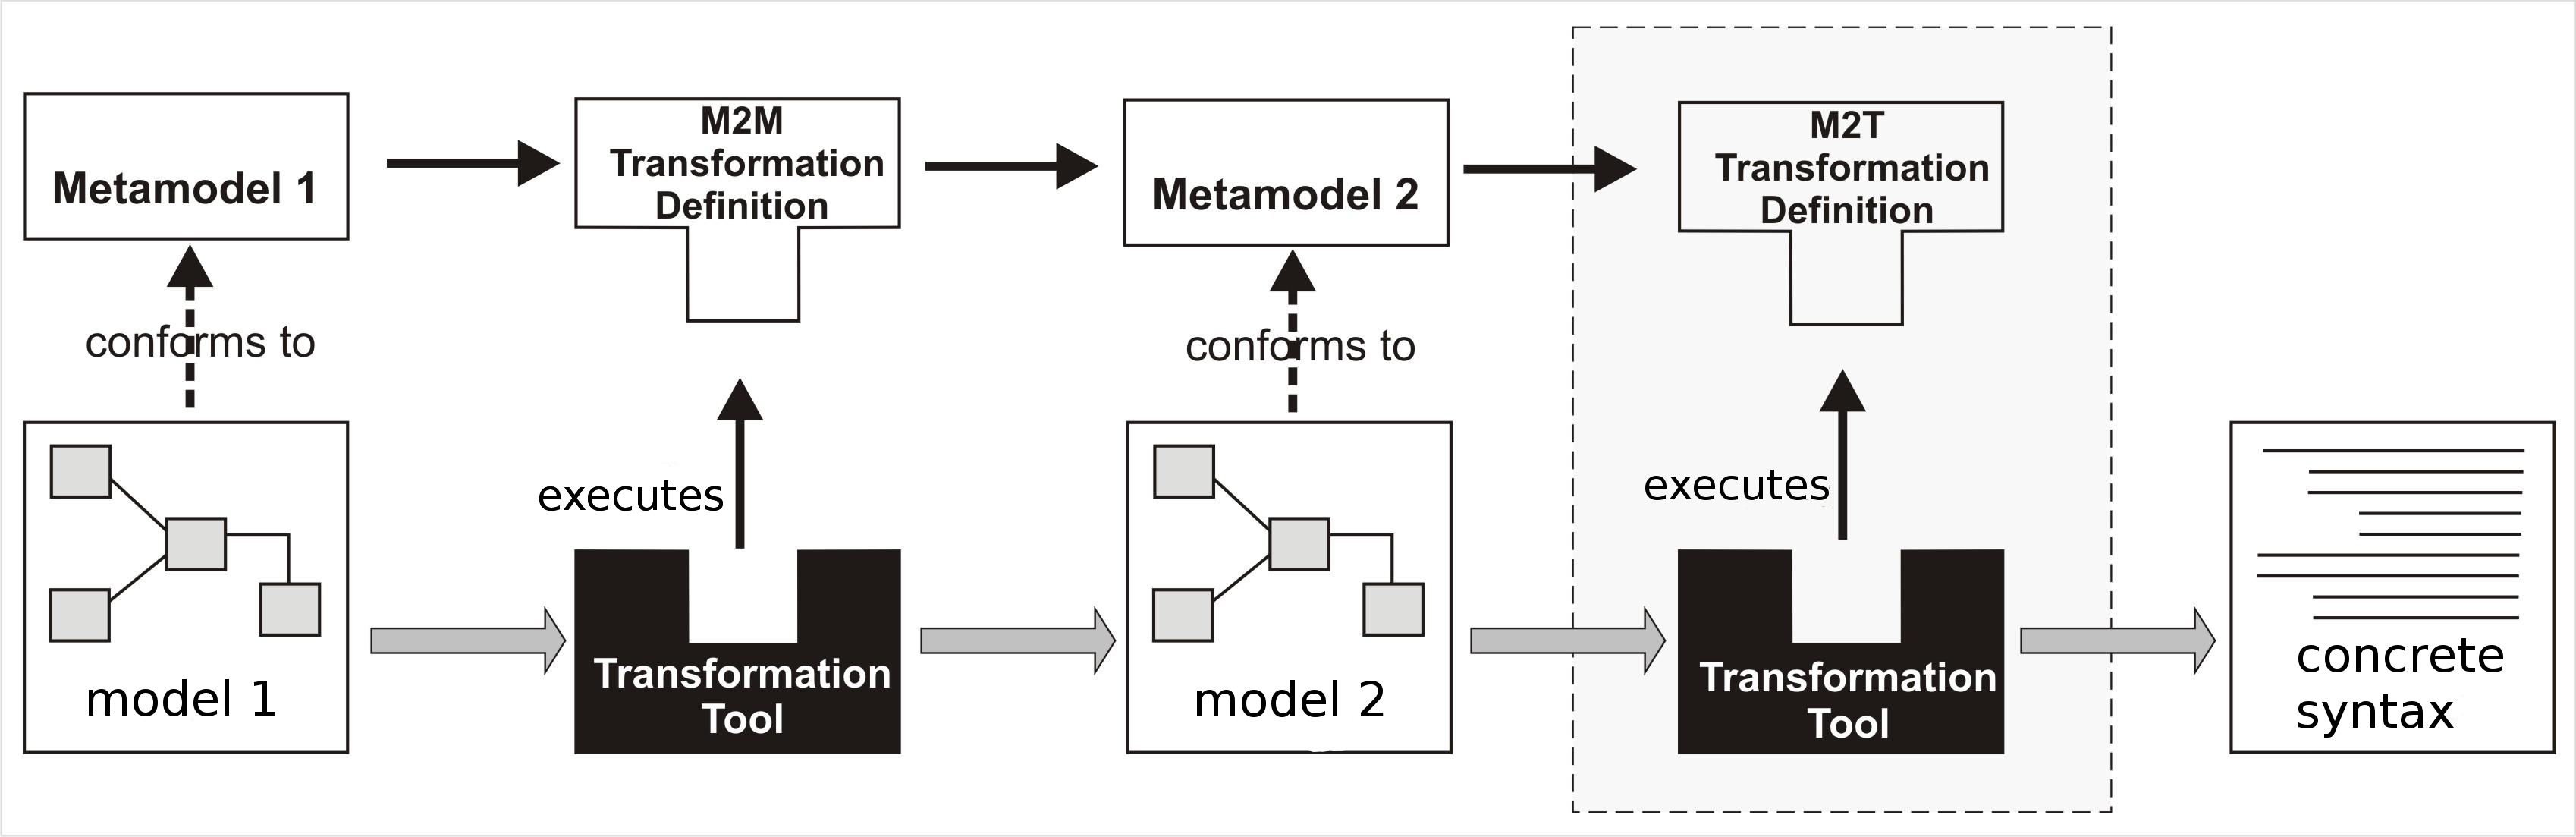
\includegraphics[scale=.12]{mdaframework}
	\caption{A simplified view of the MDD approach.}
	\label{mdaframework}
	\end{center}
\end{figure}


Apesar de algumas similaridades entre os dois tipos de transforma��es, as transforma��es entre modelos (M2M) s�o essencialmente diferentes das transforma��es de modelo para texto (M2T). As primeiras usam pelo menos dois metamodelos (um que representa os conceitos dos modelos de entrada e outro que representa os conceitos dos modelos de sa�da) e elas s�o frequentemente escritas com linguagens h�bridas, tais quais ATL \cite{atl}. Por outro lado, as transforma��es M2T comumente usam apeas um metamodelo para representar os conceitos de um modelo de entrada e elas s�o frequentemente escritas em linguagens imperativas, tais quais MOFScript e MOF2Text.


\subsection{MOFScript}

MOFScript is a language for specifying model-to-text transformations. It has many facilities that allow navigating and querying on models in order to extract data and transform them into text. It can be used to generate any kind of text, such as source code, documentation or markup languages. It took part in the process of standardization that put forward the OMG MOF Models To Text (MOF2Text or MOFM2T) specification~\cite{mof2text}. Despite some minor differences, MOF2Text and MOFScript are closely aligned.


At the time MetaTT started to be conceived, a MOF2Text language implementation, such as Acceleo, was not still available and hence our approach was elaborated on top of the MOFScript tool. Currently, Acceleo is available, but we still consider MOFScript a more robust tool for our approach and it has been widely used by the MDD community for writing model-to-text transformations. Furthermore, it has a close semantics to the MOF2Text language. It is also important to emphasize that according to the Acceleo project plan, available in~\cite{acceleo_plan}, it still has not reached the advanced feature compliance level, as specified in~\cite{mof2text}. It means that important features, such as module extension, template overriding, text mode switching and macros, are not fully implemented, what still precludes us to realize the concepts discussed in this work into the MOF2Text language. 

Concerning the language features, MOFScript offers mechanisms for abstraction and code reuse, such as inheritance, and OCL-like constructs that allow navigating on the models. On the other hand, unlike XPand and Epsilon, the MOFScript environment does not directly support the integration of its transformations into a transformation workflow, but it can be accomplished by means of its API. 

For all these reasons, we have chosen to adopt MOFScript in our approach, mainly due to its alignment with the MOF2Text standard, essential to facilitate a future migration to Acceleo.

In MOFScript, a transformation is specified by means of a \textit{texttransformation} definition that comprises import declarations, a name, the definition of the input metamodel, some properties, variables and a set of rules. Fig.~\ref{mofscriptexample} illustrates a model-to-text transformation named \texttt{JavaTT}. At line 1, an auxiliary model-to-text transformation called \texttt{JavaTexttransformation}, which is located in the package \texttt{utilPkg}, is imported. This means that all its rules can be used inside the model-to-text transformation \texttt{JavaTT}. At line 3, there is the model-to-text transformation declaration, named as \texttt{JavaTT} whose input metamodel is \texttt{"Java"}, being referenced inside the transformation as \texttt{J}. Lines 4-5 state the definition of a property and a variable, respectively. A property holds a constant value, while a variable can hold different values along transformations. Both can be declared with a global (as \texttt{version} at line 5) or local scope (as \texttt{typeDeclarations} at line 7). This latter is declared inside \textit{getCompilationUnitCode()} rule.


MOFScript rules are similar to functions, when they have a return type, or similar to procedures, when they do not. As MOFScript is a metamodel-based text transformation language, its rules may have a context type, which is a model type to which the rule is applied. A rule also may have a return type, which can be one of the built-in MOFScript types (\textit{e.g.}, \textit{String}, \textit{Real}, etc.) or a model type. Parameters can be declared too. In Fig.~\ref{mofscriptexample}, a rule is illustrated at lines 6-9. This rule returns a String value and it must be applied to instances of the \texttt{J.CompilationUnit}, which is its context type. In addition, whenever a MOFScript rule needs to return a value it must use an implicit variable, called \texttt{result}, to which the result of the computation must be assigned, as illustrated at line 8.



Two other rules are shown in Fig.~\ref{mofscriptexample}. The rule named \texttt{toFile()} at lines 10-13 is responsible for persisting strings into a file. You can note that its context is not a type, but the model-to-text transformation in which it is defined. This is specified by the keyword \texttt{module} before the rule name and means the rule can be invoked from anywhere in the transformation without the need of a context type. In this rule there are the declarations of the parameters d (the directory to which the file should be saved), v (the value of the version of the file that will be saved) and code (the code to be stored), where v ranges values of Real type, while the remaining ones range values of String type. The rule named \texttt{main} at lines 14-17 is a special rule since it is always the first one to be executed in a model-to-text transformation and hence is called an \textit{entry point} rule. Every model-to-text transformation just can be directly executed if it has a main rule. This rule can have the model-to-text transformation as its context, specified by the \texttt{module} keyword, or it can have a metamodel element as its calling context. When the context of a main rule is a metamodel element, the rule will be executed for every model element matching to this metaelement. For instance, in Fig.~\ref{mofscriptexample} the main rule is executed for every \textit{CompilationUnit} element occurring in the input model.



\footnotetext[1]{A package is implemented in MOFScript language as directories in the local file system.}


\begin{figure}[ht!]
\begin{mofscript}
\begin{lstlisting}[frame=single]
import ``utilPkg/JavaTexttransformation.m2t''

texttransformation JavaTT(in J:``Java''){
 property dir : String = ``/genCode''
 var version : Real = 1.0
 J.CompilationUnit::getCompilationUnitCode():String{
  var typeDeclarations: String = self.getTDCode()
  result = typeDeclarations
 }
 module::toFile(d: String, v: Real, code : String){ 
  file(d+``JavaFile''+v+``.java'') 
  println(code)
 }
 J.CompilationUnit::main(){
  var code: String = self.getCompilationUnitCode()
  toFile(dir, version, code)
 } 
... 
}
\end{lstlisting}
\end{mofscript}
\caption{A MOFScript transformation example.}
\label{mofscriptexample}
\end{figure}

\subsection{Ecore}


OMG has defined MOF as the standard metalanguage for specifying and managing metamodels. For accomplishing this task, Eclipse Modeling Framework (EMF) [20] has implemented a practical subset of MOF, called Ecore. Afterwards, EMF had been a significant contributor for the Essentials MOF (EMOF) that is part of the MOF2 standard [21]. This has led to a close alignment between Ecore and EMOF concepts. Since every MOF2 model can be represented as an EMOF model, it is reasonable to say that Ecore and MOF2 are aligned too.


As MOFScript is built upon EMF, it uses Ecore metamodels. Thus, our approach consequently addresses the writing of M2T generators for metamodels described with Ecore.

\begin{figure}[ht!]
  \begin{center}	
	  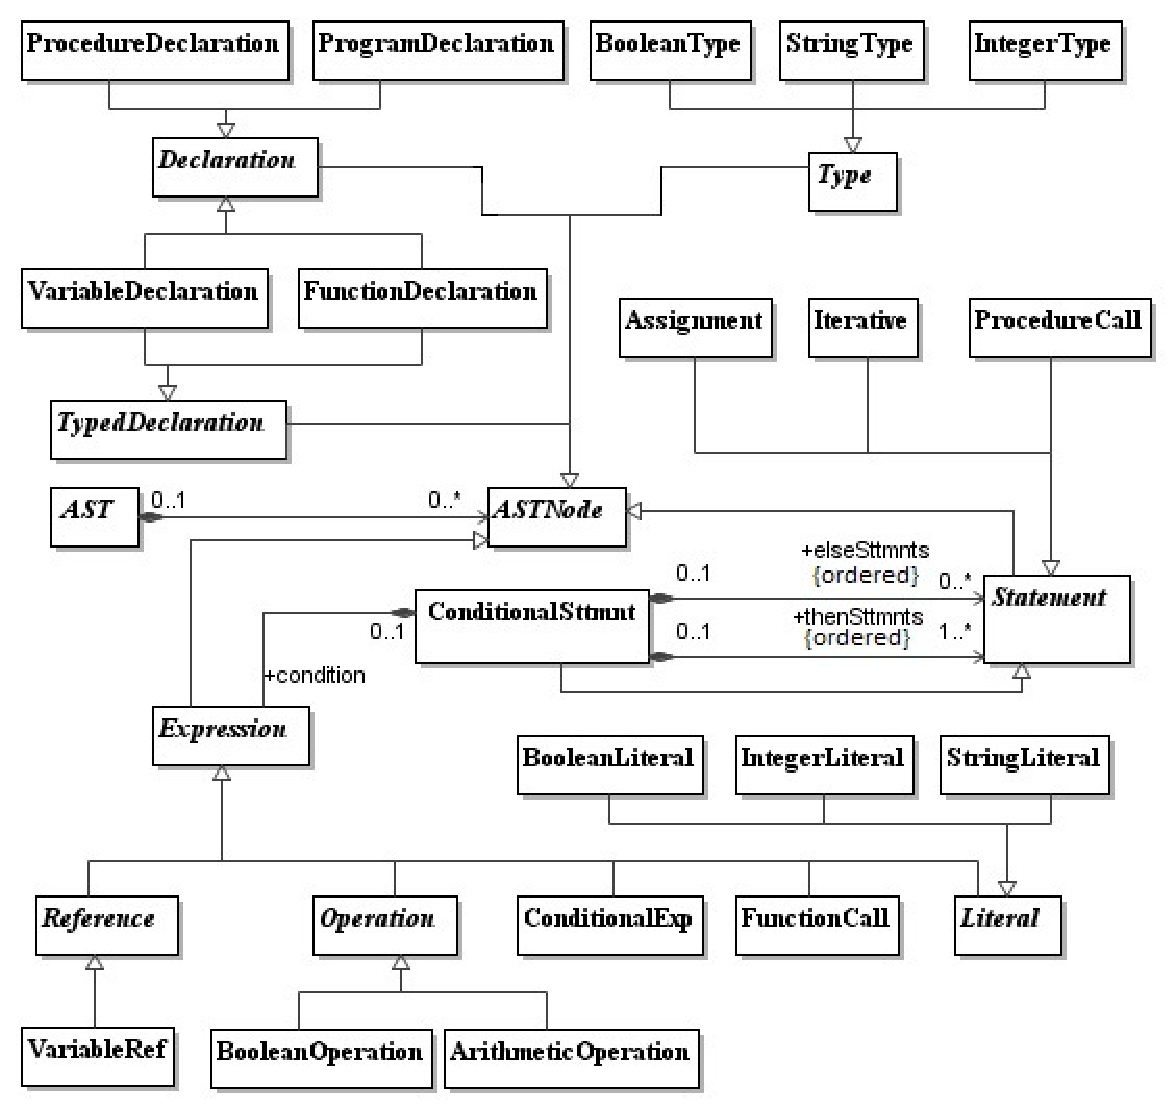
\includegraphics[scale=.425]{plang_metamodel_2}
	  \caption{PLang metamodel.}
	  \label{plangmetamodel}
  \end{center}
\end{figure}


In order to illustrate an application scenario of our approach, we have defined PLang, a simplified metamodel that mirrors simple programming language concepts. It is shown in Fig.~\ref{plangmetamodel}, where, in order to maintain simplicity, just a few composition relationships are shown. PLang metamodel works as follows:
\begin{itemize}
\item
PLang models (\textit{AST}) are composed of a set of nodes (\textit{ASTNode}). As in many procedural programming languages, PLang supports statements (\textit{Statement}), expressions (\textit{Expression}), declarations (\textit{Declaration}), types (\textit{Type}) and type declarations (\textit{TypedDeclaration}).
\item 
A statement may be further classified as an iterative statement (\textit{Iterative}), an assignment (\textit{Assignment}), a procedure call (\textit{ProcedureCall}) or a conditional statement (\textit{ConditionalSttment}).
\item 
In PLang, one can declare functions (\textit{FunctionDeclaration}), programs (\textit{ProgramDeclaration}), variables (\textit{VariableDeclaration}) and procedures (\textit{ProcedureDeclaration}).
\item
\textit{TypedDeclaration} may be classified either as (1) a \textit{VariableDeclaration} referring to the type of the values held by a variable; or as (2) a \textit{FunctionDeclaration} referring to the type of the values returned as its result.
\item
An expression in PLang is further classified as an operation (\textit{Operation}), a literal (\textit{Literal}), a function call (\textit{FunctionCall}), a reference (\textit{Reference}) or a conditional expression (\textit{ConditionalExp}).
\item
In this example, PLang supports only variable references (\textit{VariableRef}).
\item
Two kinds of operations are supported: boolean \\(\textit{BooleanOperation}) and arithmetic (\textit{ArithmeticOperation}).
\item
Three kinds of literals may appear as PLang expressions: \textit{StringLiteral}, \textit{BooleanLiteral} and \textit{IntegerLiteral} that models string, boolean and integer literals, respectively.
\item
In PLang, a \textit{ConditionalSttmnt} is composed of (i) a \textit{condition} that is an \textit{Expression}; (ii) an ordered set of statements to be executed when the condition evaluates to true, the \textit{thenSttmnts}; and, optionally, (iii) an ordered set of statements to be executed when the condition evaluates to false, the \textit{elseSttmnts}. Similarly, a \textit{FunctionCall} can have any number of arguments and a \textit{ProgramDeclaration} is composed of other declarations. However, in order to maintain simplicity just the composing relationships involving the \textit{ConditionalSttment} metaclass are illustrated.
\end{itemize}


For the sake of simplicity, some associations and compositions are not shown in Fig.~\ref{plangmetamodel}. For instance, a \textit{TypedDeclaration} has an association with a \textit{Type} and an \textit{Assignment} is composed of a \textit{VariableRef} and an \textit{Expression}. However, showing such associations and compositions would add details to Fig.~\ref{plangmetamodel} that are not essential for understanding it as well as for understanding our approach.

% END OF SECTION:  BACKGROUND

\chapter{Introdu\c{c}\~{a}o}

\section{Se\c{c}\~{a}o 1 do Cap�tulo 1}
\subsection{Subse��o}
\subsubsection{Subsubse��o}

A Figura \ref{fig:sistemaProposto}. A Tabela \ref{tab:tabelaTeste}. A Equa��o (\ref{eq1}). O trabalho de fulano~\cite{ref1}. O C�digo Fonte \ref{cod1}.



\begin{table}[htpb]
\begin{center}
\begin{tabular}{|c|c|c|}
\hline
coluna 1 & coluna 2 & coluna 3 \\
\hline
valor 1,1 & valor 1,2 & valor 1,3 \\
valor 2,1 & valor 2,2 & valor 2,3 \\
\hline
\end{tabular}
\end{center}
\caption{Primeira tabela.}
\label{tab:tabelaTeste}
\end{table}

\begin{equation}
E = m \times c^2
\label{eq1}
\end{equation}

\begin{lstlisting}[caption={Loop simples},label=cod1,numbers=none]
for(int x=1; x<10; x++){
  cout << x << "\n";
}
\end{lstlisting}

\section{Se\c{c}\~{a}o 2 do Cap�tulo 1}  
\subsection{Subse��o}
\subsubsection{Subsubse��o}




%%%%%%%%%%%%%%%%%%%%%%%%%%%%%%%%%%%%%%%%%%%%%%%%%%%%%%%%%%%%%%%%%%%%%%%%%%%%%%%%
%% BIbliografia
%% Coloque suas referencias no arquivo ref.bib e descomente as proximas duas linhas

\bibliographystyle{plain} % estilo de bibliografia   plain,unsrt,alpha,abbrv.
\bibliography{ref} % arquivos com as entradas bib.

%%%%%%%%%%%%%%%%%%%%%%%%%%%%%%%%%%%%%%%%%%%%%%%%%%%%%%%%%%%%%%%%%%%%%%%%%%%%%%%%
%% Apendice
% Caso seja necessario algum apendice, descomente a proxima linha.

\appendix
\chapter{Meu primeiro ap�ndice}

\chapter{Meu segundo ap�ndice}

%%%%%%%%%%%%%%%%%%%%%%%%%%%%%%%%%%%%%%%%%%%%%%%%%%%%%%%%%%%%%%%%%%%%%%%%%%%%%%%%

\end{document}